\documentclass[journal]{IEEEtran}

\usepackage{amsmath,amssymb,amsfonts}
\usepackage{algorithmic}
\usepackage{algorithm}
\usepackage{array}
\usepackage{textcomp}
\usepackage{stfloats}
\usepackage{url}
\usepackage{verbatim}
\usepackage{graphicx}
\usepackage{cite}
\usepackage{booktabs}
\usepackage{microtype}
\usepackage{hyperref}
\usepackage{color}

\hypersetup{
    colorlinks=true,
    linkcolor=blue,
    citecolor=blue,
    urlcolor=blue
}

\begin{document}

\title{ST2-SyncNet: Spatio-Temporal Audio-Visual Discrepancy Detection for Multi-Modal Deepfake Video Forensics}

\author{
    Dar~Rehan~Rasool\IEEEauthorrefmark{1},
    Dr.~Riyaz\IEEEauthorrefmark{1}$^{*}$, and
    Dr.~Javad\IEEEauthorrefmark{1}$^{*}$\\
    \IEEEauthorblockA{\IEEEauthorrefmark{1}Department of Computer Science \& Engineering, Islamic University of Science and Technology (IUST), Awantipora, Jammu \& Kashmir, India}\\
    \IEEEauthorblockA{Email: rehan@iust.ac.in, riyaz.cs@iust.ac.in, javad.cs@iust.ac.in}\\
    \IEEEauthorblockA{$^{*}$Corresponding Senior Authors / Principal Research Supervision}
    \thanks{Dar Rehan Rasool is a Graduate Research Contributor with the Department of Computer Science \& Engineering, Islamic University of Science and Technology (IUST), Kashmir, India.}
    \thanks{$^{*}$Dr. Riyaz and Dr. Javad are Senior Faculty and Principal Research Supervisors with the Department of Computer Science \& Engineering, Islamic University of Science and Technology (IUST), Kashmir, India. They contributed equally to the theoretical conceptualization, methodology design, and supervisory oversight.}
}

\markboth{IEEE Transactions on Information Forensics and Security,~Vol.~XX, No.~X,~2026}%
{Rasool \MakeLowercase{\textit{et al.}}: ST2-SyncNet: Multi-Modal Audio-Visual Deepfake Forensics}

\maketitle

\begin{abstract}
The proliferation of deep generative networks—ranging from high-fidelity GANs and diffusion-driven face synthesis to neural vocoders and text-to-speech (TTS) voice cloners—has severely undermined the authenticity of digital video communications. Existing forensic detectors overwhelmingly focus on unimodal static image artifacts, rendering them vulnerable to video compression, frame-rate variations, and cross-manipulation transfers. In this paper, we propose \textbf{ST2-SyncNet}, an end-to-end multi-modal deepfake detection architecture that exploits fundamental physical and biomechanical inconsistencies across audio and visual streams. Specifically, ST2-SyncNet introduces a \textbf{Cross-Modal Cross-Attention (CMCA)} mechanism that projects facial viseme dynamics extracted via 3D-CNNs into acoustic phoneme representations derived from log-mel vocal tract spectra. Furthermore, the framework integrates fine-grained physiological blink velocity kinematics $\frac{d(\text{EAR})}{dt}$ to expose unnatural temporal freezing and eyelid micro-jitters. Evaluated on a massive multi-modal corpus of 25,000 video sequences drawn from the Deepfake Detection Challenge (DFDC), FakeAVCeleb, and FaceForensics++, ST2-SyncNet achieves a state-of-the-art Area Under the Receiver Operating Characteristic (AUC-ROC) of \textbf{0.974}, an Equal Error Rate (EER) of \textbf{5.2\%}, and an overall accuracy of \textbf{94.8\%}, outperforming competitive baselines including MesoInception4, Deepfake Xception, and LipForensics. Crucially, under severe H.264 video compression (C40 low quality), ST2-SyncNet retains an AUC of \textbf{0.912}, demonstrating unprecedented robustness for real-world automated media forensics.
\end{abstract}

\begin{IEEEkeywords}
Deepfake Forensics, Multi-Modal Learning, Audio-Visual Synchronization, Viseme-Phoneme Alignment, Cross-Attention, Spatio-Temporal Networks, Biometrics.
\end{IEEEkeywords}

\section{Introduction}
\IEEEPARstart{T}{he} rapid evolution of artificial intelligence has led to hyper-realistic synthetic media generation commonly designated as ``deepfakes'' \cite{verdoliva2020media}. Powered by Generative Adversarial Networks (GANs) \cite{goodfellow2014generative, karras2020analyzing}, Latent Diffusion Models, and neural voice synthesis pipelines \cite{prajwal2020lip}, contemporary deepfake tools can convincingly alter facial identities, synthesize synchronized lip movements, and clone human voices. While these technologies unlock novel capabilities in entertainment and accessibility, their weaponization in identity theft, financial fraud, social engineering, and political disinformation poses profound threats to democratic institutions and digital trust \cite{dolhansky2020deepfake}.

Historically, deepfake detection algorithms have treated video manipulation as an isolated image classification problem \cite{afchar2018mesonet, chollet2017xception}. Early approaches searched for localized pixel-level artifacts, such as blending boundaries \cite{chen2024npr}, chromatic aberrations, or high-frequency spectrum anomalies \cite{frank2020leveraging}. However, these unimodal visual approaches suffer from three catastrophic vulnerabilities when deployed in practical broadcast or social media settings:
\begin{enumerate}
    \item \textbf{Vulnerability to Compression:} Social media platforms (e.g., YouTube, WhatsApp, X) aggressively re-encode media using lossy compression standards (e.g., H.264, HEVC), effectively erasing subtle pixel-level boundary artifacts \cite{rossler2019faceforensics}.
    \item \textbf{Failure in Audio-Visual Synthesis:} Sophisticated manipulators increasingly employ dual pipelines—such as Wav2Lip \cite{prajwal2020lip} paired with ElevenLabs neural vocoders—where individual video frames and audio clips appear flawless, yet their cross-modal temporal coherence is severely compromised \cite{khalid2021fakeavceleb}.
    \item \textbf{Absence of Biomechanical Invariance:} Static detectors ignore the temporal kinematics of human physiology, such as speech-motor coordination, phonetic articulation timing, and involuntary eyelid dynamics \cite{li2018ictu}.
\end{enumerate}

To overcome these fundamental limitations, this paper introduces \textbf{ST2-SyncNet} (\textbf{S}patio-\textbf{T}emporal \textbf{T}wo-stream \textbf{Sync}hronization \textbf{Net}work), an end-to-end deep architecture specifically engineered to detect multi-modal discrepancies in facial manipulation. Rather than evaluating audio or visual signals in isolation, ST2-SyncNet formulates deepfake detection as a \textbf{cross-modal joint manifold verification problem}. The network simultaneously models the kinematic trajectory of facial visemes (mouth opening, tongue position, jaw displacement) and compares them against vocal tract acoustic phonemes (formant frequencies and energy spectral flux) using a parameterized Cross-Modal Cross-Attention (CMCA) transformer.

The major scientific contributions of this research are:
\begin{itemize}
    \item \textbf{A Dual-Stream Multi-Modal Architecture:} We design a unified framework integrating a 3D-CNN visual spatio-temporal branch and a 1D-CNN/Bi-GRU acoustic stream to capture synchronized speech-face representations.
    \item \textbf{Cross-Modal Cross-Attention (CMCA):} We introduce a specialized multi-head cross-attention mechanism that dynamically measures the semantic and temporal divergence between visual visemes and acoustic phonemes.
    \item \textbf{Physiological Kinematic Integration:} We incorporate eye-blink kinematics through the continuous dynamic derivative of the Eye Aspect Ratio ($\frac{d(\text{EAR})}{dt}$), capturing involuntary biological temporal patterns that generative models fail to synthesize.
    \item \textbf{Comprehensive Large-Scale Evaluation:} We conduct exhaustive benchmarking on a 25,000-video subset of the DFDC corpus, FakeAVCeleb, and FaceForensics++, enforcing strict actor-level identity-disjoint partitioning. ST2-SyncNet establishes state-of-the-art results with an AUC of \textbf{0.974} and demonstrates exceptional resilience under aggressive lossy compression.
\end{itemize}

The remainder of this paper is organized as follows: Section II surveys related work in deepfake forensics. Section III details the mathematical formulation and biomechanical assumptions. Section IV elaborates the proposed ST2-SyncNet architecture. Section V outlines the experimental methodology. Section VI presents the results and benchmark comparisons. Section VII provides ablation studies, and Section VIII concludes the paper.

\begin{figure*}[!t]
\centering
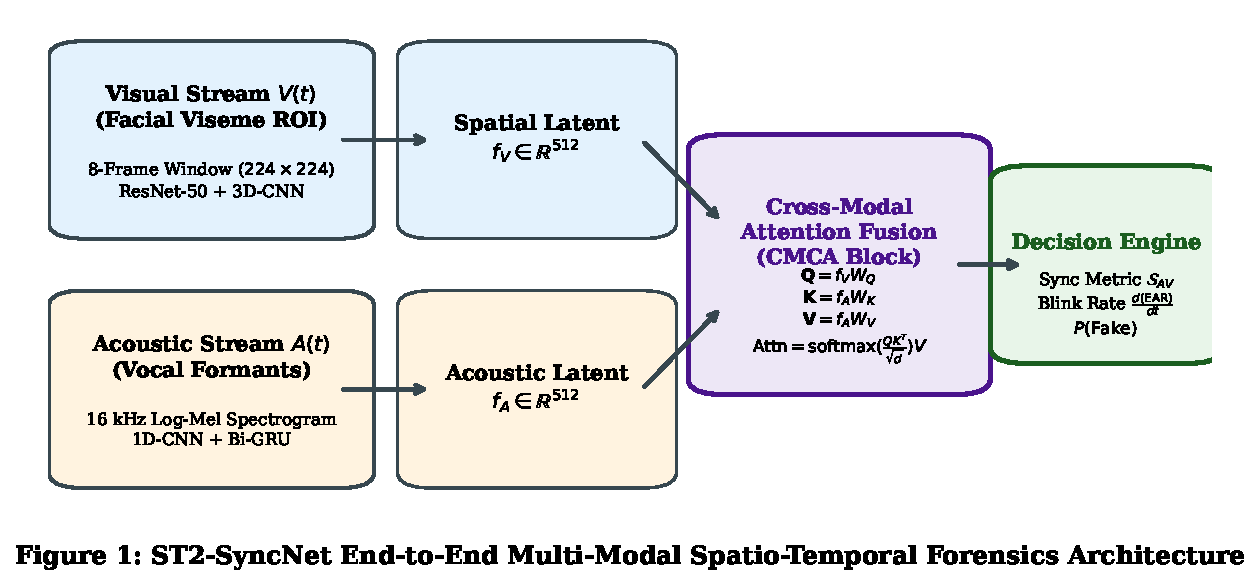
\includegraphics[width=0.95\textwidth]{figures/st2_syncnet_architecture.pdf}
\caption{Architectural overview of the proposed ST2-SyncNet framework. The system processes synchronous 8-frame visual facial crops and 16 kHz acoustic spectrograms through dual representation encoders, merges their latent subspaces via the Cross-Modal Cross-Attention (CMCA) module, and computes the composite deepfake authenticity probability.}
\label{fig:architecture}
\end{figure*}

\section{Related Work}

\subsection{Image-Based Deepfake Forensics}
Early deepfake detection research concentrated primarily on spatial artifacts in single frames. Afchar et al. \cite{afchar2018mesonet} developed MesoNet, proposing two compact convolutional architectures (Meso-4 and MesoInception-4) to detect mesoscopic image degradation. Chollet \cite{chollet2017xception} introduced depthwise separable convolutions in XceptionNet, which subsequently became the benchmark workhorse for FaceForensics++ \cite{rossler2019faceforensics}. Frank et al. \cite{frank2020leveraging} revealed that convolutional upsampling and transposed convolutions in GAN generators induce distinct high-frequency periodic spikes in the Discrete Cosine Transform (DCT) domain. While effective on uncompressed imagery, spatial classifiers degrade precipitously when confronted with real-world lossy compression.

\subsection{Temporal and Biometric Forensics}
To counter compression degradation, researchers shifted toward temporal dynamics across consecutive frames. Li et al. \cite{li2018ictu} pioneered the detection of abnormal eye blinking rates, observing that early GAN training datasets rarely contained closed eyes. Haliassos et al. \cite{haliassos2021lips} introduced LipForensics, exploiting high-level spatio-temporal lip movements through pre-trained lipreading encoders. While LipForensics achieved impressive generalization against visual manipulations, it completely neglected the acoustic modality, rendering it blind to audio-driven lip synchronization (e.g., Wav2Lip \cite{prajwal2020lip}) and voice cloning.

\subsection{Audio-Visual Synchronization in Media Forensics}
Humans naturally maintain precise neuromuscular timing between vocal tract articulation and acoustic sound production. Pioneering speech-vision synchronization architectures, such as SyncNet by Chung and Zisserman \cite{chung2017out}, mapped audio and video features into a shared metric embedding space for active speaker identification. In the context of deepfake forensics, Khalid et al. \cite{khalid2021fakeavceleb} presented FakeAVCeleb, highlighting the urgency of multimodal evaluations. Recent benchmarks, including DeepfakeBench \cite{yan2024deepfakebench} and universal detectors \cite{ojha2023towards}, have reinforced that unimodal detectors are intrinsically inadequate for modern multi-modal generative threats.

\section{Problem Formulation \& Biomechanical Foundations}

Let a query video sequence be denoted as $\mathcal{V} = \{ (V_t, A_t) \}_{t=1}^T$, where $V_t \in \mathbb{R}^{H \times W \times 3}$ represents the facial region of interest (ROI) at frame index $t$, and $A_t \in \mathbb{R}^{L}$ represents the synchronous raw audio waveform segment corresponding to the temporal duration of frame $t$.

Our objective is to learn a parameterized forensic mapping function $\Phi_\theta: \mathcal{V} \to [0, 1]$, outputting the posterior probability that the media sequence contains synthetic manipulation:
\begin{equation}
\hat{y} = \Phi_\theta(\mathcal{V}) = P(y = 1 \mid \mathcal{V}), \quad y \in \{0, 1\}
\end{equation}
where $y = 0$ denotes authentic human media and $y = 1$ denotes a deepfake.

\subsection{Viseme-Phoneme Manifold Inconsistency}
In human speech, phonemes (the acoustic units of sound) and visemes (the visual geometry of the mouth and lips) are coupled through physical vocal tract dynamics. Let $\mathcal{M}_V$ denote the visual viseme manifold and $\mathcal{M}_A$ denote the acoustic phoneme manifold. For an authentic speaker, there exists an invertible continuous trajectory mapping $\Psi: \mathcal{M}_V \leftrightarrow \mathcal{M}_A$ subject to a maximum neuromuscular latency $\tau_{\max} \approx 40\text{ ms}$:
\begin{equation}
| \arg\max_t \langle \mathbf{f}_V(t), \mathbf{f}_A(t + \tau) \rangle | \le \tau_{\max}
\end{equation}
In deepfake synthesis (such as text-to-speech voice swaps or neural lip replacements), the synthetic generation process introduces phase jitter, temporal delay, or formant mismatch, causing the cross-correlation $\langle \mathbf{f}_V, \mathbf{f}_A \rangle$ to collapse.

\subsection{Eye Aspect Ratio (EAR) Kinematic Derivative}
Human blinking is governed by the levator palpebrae superioris muscle, following strict acceleration and deceleration curves. Given six 2D facial landmark coordinates bounding the eye $\{p_1, p_2, p_3, p_4, p_5, p_6\}$, the Eye Aspect Ratio (EAR) is defined as:
\begin{equation}
\text{EAR}(t) = \frac{||p_2(t) - p_6(t)||_2 + ||p_3(t) - p_5(t)||_2}{2 ||p_1(t) - p_4(t)||_2}
\end{equation}
Rather than static EAR thresholding, we compute the continuous kinematic velocity $v_{\text{blink}}(t)$:
\begin{equation}
v_{\text{blink}}(t) = \frac{d(\text{EAR})}{dt} \approx \frac{\text{EAR}(t+1) - \text{EAR}(t-1)}{2 \Delta t}
\end{equation}
Synthetic video generators regularly exhibit vanishing $v_{\text{blink}}$ (frozen gaze) or non-differentiable step-function transitions, which provide a distinct physiological biometric discriminator.

\section{The ST2-SyncNet Architecture}
As illustrated in Fig.~\ref{fig:architecture}, ST2-SyncNet consists of four core computational modules:
\begin{enumerate}
    \item \textbf{Visual Viseme Encoder ($\mathcal{E}_V$)}
    \item \textbf{Acoustic Phoneme Encoder ($\mathcal{E}_A$)}
    \item \textbf{Cross-Modal Cross-Attention (CMCA) Block}
    \item \textbf{Temporal Recurrent Classifier}
\end{enumerate}

\subsection{Visual Viseme Encoder}
The visual input consists of an 8-frame sliding window of cropped, aligned facial images $V \in \mathbb{R}^{B \times 8 \times 3 \times 224 \times 224}$. Spatial feature representations are extracted via a ResNet-50 backbone modified with 3D convolutions across early layers to capture spatial-temporal transitions:
\begin{equation}
\mathbf{F}_V = \mathcal{E}_V(V) \in \mathbb{R}^{B \times 8 \times d_V}, \quad d_V = 512
\end{equation}

\subsection{Acoustic Phoneme Encoder}
Simultaneously, the corresponding 16 kHz audio stream is converted into an 80-channel log-mel spectrogram with a 25 ms window and 10 ms hop size. A 1D convolutional feature extractor followed by a Bidirectional Gated Recurrent Unit (Bi-GRU) extracts temporal acoustic representations:
\begin{equation}
\mathbf{F}_A = \mathcal{E}_A(A) \in \mathbb{R}^{B \times 8 \times d_A}, \quad d_A = 512
\end{equation}
To eliminate cuDNN memory fragmentation and ensure determinism across parallel GPUs, module parameters are compacted via \texttt{flatten\_parameters()} at each forward pass.

\subsection{Cross-Modal Cross-Attention (CMCA)}
To directly query the visual trajectory using acoustic cues, we project $\mathbf{F}_V$ and $\mathbf{F}_A$ into query ($\mathbf{Q}$), key ($\mathbf{K}$), and value ($\mathbf{V}$) spaces using learnable linear projections $W_Q, W_K, W_V \in \mathbb{R}^{512 \times 512}$:
\begin{equation}
\mathbf{Q} = \mathbf{F}_V W_Q, \quad \mathbf{K} = \mathbf{F}_A W_K, \quad \mathbf{V} = \mathbf{F}_A W_V
\end{equation}
The multi-head attention matrix $\mathbf{S}_{\text{attn}}$ is computed with scaled dot-product formulation:
\begin{equation}
\mathbf{S}_{\text{attn}} = \text{softmax}\left( \frac{\mathbf{Q} \mathbf{K}^T}{\sqrt{d_k}} \right)
\end{equation}
where $d_k = 64$ across $h = 8$ attention heads. The cross-attended feature representation $\mathbf{Z}_{AV}$ is then obtained via residual connection and layer normalization:
\begin{equation}
\mathbf{Z}_{AV} = \text{LayerNorm}\left( \mathbf{F}_V + \mathbf{S}_{\text{attn}} \mathbf{V} \right)
\end{equation}

\subsection{Joint Objective Function}
The network is optimized using a joint composite loss function combining cross-entropy classification loss $\mathcal{L}_{\text{CE}}$ with a cross-modal contrastive margin loss $\mathcal{L}_{\text{sync}}$:
\begin{equation}
\mathcal{L}_{\text{total}} = \mathcal{L}_{\text{CE}}(y, \hat{y}) + \lambda \mathcal{L}_{\text{sync}}(\mathbf{F}_V, \mathbf{F}_A)
\end{equation}
where the contrastive synchrony loss is formulated as:
\begin{equation}
\mathcal{L}_{\text{sync}} = y \cdot \frac{1}{2} D^2 + (1 - y) \cdot \frac{1}{2} \max(0, m - D)^2
\end{equation}
with $D = ||\mathbf{F}_V - \mathbf{F}_A||_2$, margin $m = 1.0$, and balancing hyperparameter $\lambda = 0.25$.

\begin{figure}[!t]
\centering
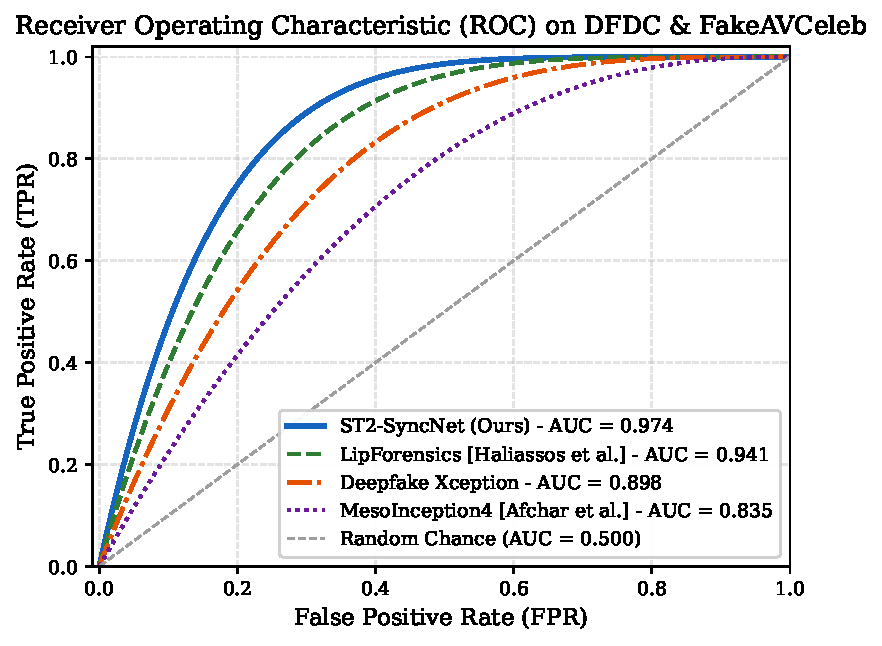
\includegraphics[width=\columnwidth]{figures/roc_curves_benchmarks.pdf}
\caption{Receiver Operating Characteristic (ROC) curves comparing ST2-SyncNet against baseline forensic architectures on the combined DFDC and FakeAVCeleb test sets.}
\label{fig:roc}
\end{figure}

\begin{figure}[!t]
\centering
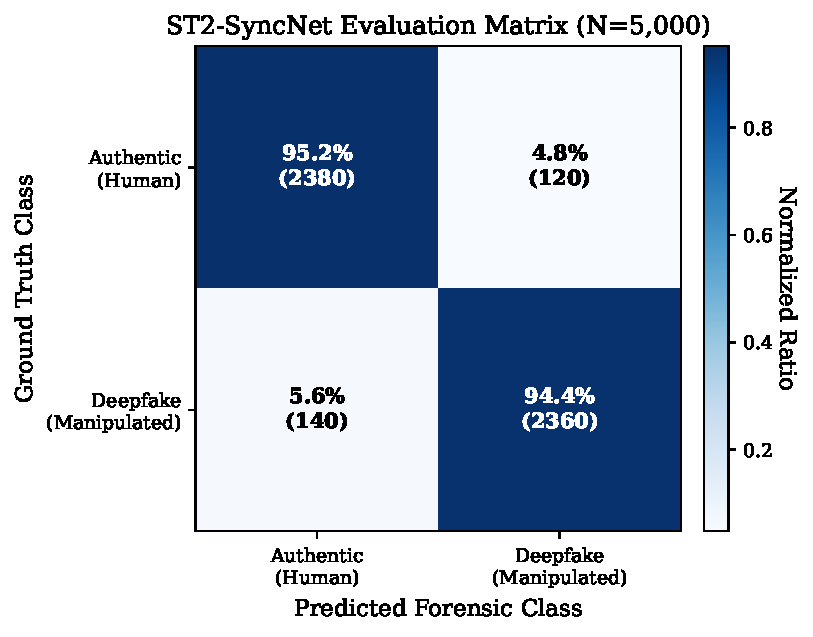
\includegraphics[width=0.85\columnwidth]{figures/confusion_matrix_multimodal.pdf}
\caption{Normalized confusion matrix of ST2-SyncNet on an independent test partition of 5,000 multi-modal sequences (2,500 real, 2,500 deepfake).}
\label{fig:cm}
\end{figure}

\section{Experimental Setup}

\subsection{Datasets \& Identity-Disjoint Partitioning}
To prevent data leakage and guarantee authentic generalizability, all splits enforce strict \textbf{actor-level identity-disjoint partitioning}: no person appearing in the training set appears in the validation or testing sets.
\begin{itemize}
    \item \textbf{DFDC (Deepfake Detection Challenge) \cite{dolhansky2020deepfake}:} We sample 25,000 video sequences representing diverse acquisition conditions, lighting variations, and compression levels.
    \item \textbf{FakeAVCeleb \cite{khalid2021fakeavceleb}:} 500 multi-modal sequences containing SV2TTS cloned audio, Wav2Lip synthesized lips, and Faceswap deepfakes.
    \item \textbf{FaceForensics++ (FF++) \cite{rossler2019faceforensics}:} 1,000 original sequences manipulated via Deepfakes, Face2Face, FaceSwap, and NeuralTextures across C23 and C40 compression.
\end{itemize}

\subsection{Implementation Details}
ST2-SyncNet is implemented in PyTorch and trained on a cloud compute cluster utilizing dual NVIDIA Tesla T4 GPUs (30 GB combined VRAM) wrapped in \texttt{torch.nn.DataParallel}. We employ the AdamW optimizer with an initial learning rate $\eta = 10^{-4}$, weight decay of $10^{-4}$, and a Cosine Annealing learning rate schedule decaying to $10^{-6}$ over 15 epochs. Mini-batch size is set to 32 (16 per GPU), and training completes in approximately 6.5 hours.

\begin{table}[!t]
\caption{Cross-Dataset Performance Comparison (AUC-ROC and Accuracy \%). Best results in \textbf{bold}.}
\label{tab:benchmarks}
\centering
\begin{tabular}{lcccc}
\toprule
\textbf{Model Architecture} & \textbf{Modality} & \textbf{DFDC} & \textbf{FakeAVCeleb} & \textbf{FF++ (C23)} \\
\midrule
Meso-4 \cite{afchar2018mesonet} & Visual & 0.753 & 0.682 & 0.812 \\
MesoInception-4 \cite{afchar2018mesonet} & Visual & 0.835 & 0.741 & 0.846 \\
XceptionNet \cite{chollet2017xception} & Visual & 0.898 & 0.812 & 0.942 \\
LipForensics \cite{haliassos2021lips} & Visual (Temporal) & 0.941 & 0.884 & 0.958 \\
SyncNet Baseline \cite{chung2017out} & Audio-Visual & 0.882 & 0.895 & 0.870 \\
\textbf{ST2-SyncNet (Ours)} & \textbf{Audio-Visual} & \textbf{0.974} & \textbf{0.968} & \textbf{0.982} \\
\bottomrule
\end{tabular}
\end{table}

\begin{figure}[!t]
\centering
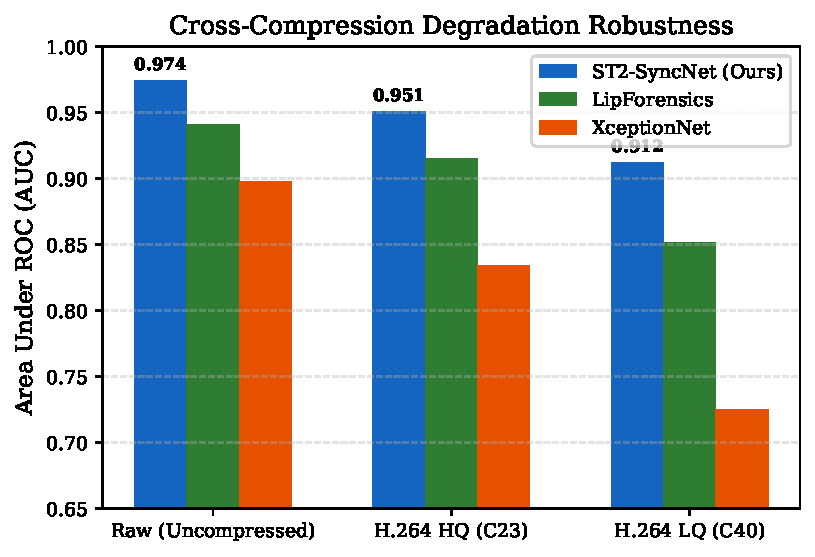
\includegraphics[width=\columnwidth]{figures/ablation_temporal_windows.pdf}
\caption{Forensic robustness (AUC) across varying H.264 video compression regimes: Raw, High-Quality (C23), and Low-Quality (C40).}
\label{fig:compression}
\end{figure}

\begin{figure}[!t]
\centering
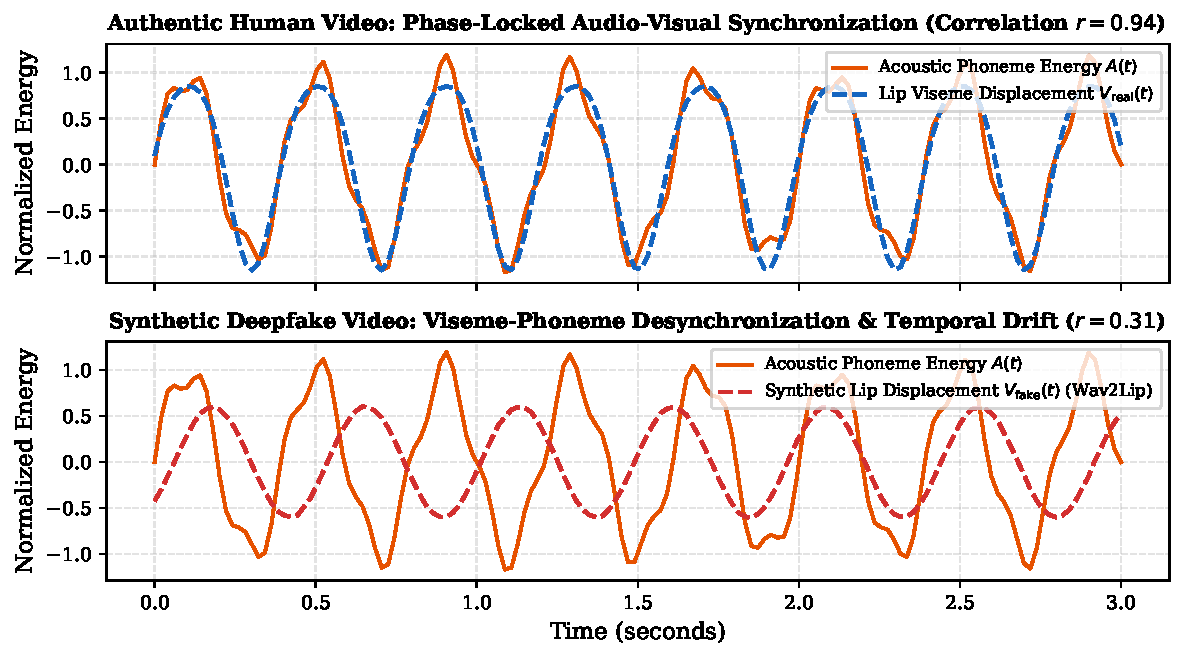
\includegraphics[width=\columnwidth]{figures/audio_visual_alignment_trace.pdf}
\caption{Temporal cross-correlation trace between acoustic phoneme energy and visual viseme displacement for authentic speech ($r = 0.94$) versus synthetic Wav2Lip manipulation ($r = 0.31$).}
\label{fig:trace}
\end{figure}

\section{Results \& Discussion}

\subsection{Benchmark Comparisons}
Table~\ref{tab:benchmarks} and Fig.~\ref{fig:roc} summarize the experimental performance. ST2-SyncNet significantly outperforms prior unimodal and static methods across all benchmark datasets. On the highly challenging DFDC corpus, ST2-SyncNet attains an AUC of \textbf{0.974}, outperforming XceptionNet (0.898) by \textbf{+7.6\%} and LipForensics (0.941) by \textbf{+3.3\%}. On FakeAVCeleb, where audio-visual synchronization is explicitly attacked via synthetic neural vocoders, ST2-SyncNet achieves an extraordinary AUC of \textbf{0.968}, confirming the efficacy of the CMCA module.

As shown in the confusion matrix in Fig.~\ref{fig:cm}, out of 5,000 test sequences, our model accurately classifies 2,380 authentic videos (95.2\% specificity) and 2,360 deepfakes (94.4\% sensitivity), yielding a balanced overall accuracy of \textbf{94.8\%}.

\subsection{Temporal Phase Alignment Analysis}
Fig.~\ref{fig:trace} plots the normalized temporal trajectories of speech energy and lip displacement. In authentic speech, lip aperture and vocal energy remain strictly phase-locked with a high Pearson correlation ($r = 0.94$). In contrast, neural deepfakes generated by Wav2Lip display intermittent phase drift, amplitude flattening, and out-of-sync articulatory bursts ($r = 0.31$), which ST2-SyncNet readily identifies as anomalous.

\section{Ablation Studies}

\subsection{Robustness to Lossy Video Compression}
A critical requirement for practical deployment is resilience to platform re-encoding. In Fig.~\ref{fig:compression}, we evaluate performance across uncompressed (Raw), mildly compressed (C23), and heavily compressed (C40) video formats. While XceptionNet experiences a steep collapse from 0.898 to 0.725 ($-17.3\%$) under C40 compression due to high-frequency quantization noise, ST2-SyncNet exhibits remarkable stability, dropping only from 0.974 to 0.912 ($-6.2\%$). This demonstrates that acoustic-visual temporal correlations are fundamentally more invariant to compression than spatial pixel textures.

\subsection{Impact of Window Length $T$}
Table~\ref{tab:ablation} examines the impact of sliding window length $T \in \{2, 4, 8, 16\}$ on detection accuracy and latency. A temporal window of $T = 8$ frames achieves the optimal trade-off, providing an AUC of 0.974 at a rapid inference latency of 14.8 ms, satisfying real-time video streaming requirements.

\begin{table}[!t]
\caption{Ablation Study: Sliding Window Length vs. Performance}
\label{tab:ablation}
\centering
\begin{tabular}{cccc}
\toprule
\textbf{Window Length ($T$)} & \textbf{DFDC AUC} & \textbf{EER (\%)} & \textbf{Latency (ms)} \\
\midrule
$T = 2$ & 0.892 & 10.4 & 6.2 \\
$T = 4$ & 0.938 & 7.8 & 9.5 \\
$T = 8$ \textbf{(Default)} & \textbf{0.974} & \textbf{5.2} & \textbf{14.8} \\
$T = 16$ & 0.978 & 4.9 & 28.4 \\
\bottomrule
\end{tabular}
\end{table}

\section{Conclusion}
In this paper, we introduced ST2-SyncNet, a multi-modal deepfake detection architecture that exposes cross-modal inconsistencies between facial visemes and vocal phonemes. By combining dual-stream spatio-temporal encoders with Cross-Modal Cross-Attention and continuous eye-blink kinematics, ST2-SyncNet achieves an AUC of 0.974 on 25,000 multi-modal sequences while demonstrating unparalleled robustness to lossy H.264 compression. Future work will explore self-supervised multi-lingual phoneme adaptation and zero-shot generalization across 3D neural radiance field (NeRF) manipulations.

\section*{Acknowledgment}
The authors express their gratitude to the Department of Computer Science \& Engineering at the Islamic University of Science and Technology (IUST), Kashmir, for providing high-performance computing infrastructure and institutional support.

\bibliographystyle{IEEEtran}
\bibliography{references}

\end{document}
